% !TEX program = lualatex
\documentclass[12pt,a4paper]{article}

% --------------------- Preamble ---------------------
\usepackage{fontspec}
\setmainfont{TeX Gyre Termes}
\usepackage{microtype}
\usepackage{geometry}
\geometry{margin=1.1in}
\usepackage{setspace}
\setstretch{1.2}
\usepackage{parskip}
\usepackage{titlesec}
\titleformat{\section}{\Large\bfseries}{\thesection.}{0.8em}{}
\titleformat{\subsection}{\large\bfseries}{\thesubsection}{0.6em}{}
\titleformat{\paragraph}[runin]{\bfseries}{\theparagraph}{0.8em}{}[.]

\usepackage{enumitem}
\setlist{topsep=4pt,itemsep=4pt}
\usepackage[hidelinks]{hyperref}
\usepackage{amsmath,amssymb,bm}
\usepackage{physics}
\usepackage{booktabs}
\usepackage{array}
\usepackage{float}
\usepackage{ragged2e}
\usepackage{xcolor}
\usepackage{amsthm}
\usepackage{makeidx}
\makeindex
\usepackage{tikz}
\usepackage{pgfplots}
\pgfplotsset{compat=1.18}

% Theorem environments
\theoremstyle{plain}
\newtheorem{theorem}{Theorem}[section]
\newtheorem{proposition}[theorem]{Proposition}
\newtheorem{lemma}[theorem]{Lemma}
\newtheorem{corollary}[theorem]{Corollary}
\theoremstyle{definition}
\newtheorem{definition}[theorem]{Definition}
\newtheorem{conjecture}[theorem]{Conjecture}
\theoremstyle{remark}
\newtheorem{remark}[theorem]{Remark}

% Small macros
\newcommand{\Phifield}{\Phi}
\newcommand{\vfield}{\mathcal{v}}
\newcommand{\Sfield}{S}
\newcommand{\AI}{\mathrm{A}}
\newcommand{\Entropy}{\mathcal{H}}

% Title block
\title{\textbf{Procedural Ontology: The Metaphysics of Code Generation}\\
\large A Relativistic Scalar--Vector Plenum (RSVP) Essay}
\author{Flyxion}
\date{2025}

% --------------------- Document ---------------------
\begin{document}
\maketitle

% --------------------- Summary of Sections ---------------------
\section*{Section Synopses}
\addcontentsline{toc}{section}{Section Synopses}
\textit{Section 1.} \textit{Text is not inert symbol but anticipatory matter, encoding potential energy as syntactic curvature within a measurable linguistic manifold.}\index{linguistic manifold}

\textit{Section 2.} \textit{Execution transforms frozen law into kinetic flow via stochastic differential equations on the linguistic manifold, linking gradient descent to Hamiltonian mechanics.}\index{execution!stochastic}

\textit{Section 3.} \textit{Rendering is entropic expansion: the diffusion of compressed potential into observable diversity, quantified by Shannon entropy over output distributions.}\index{rendering!entropy}

\textit{Section 4.} \textit{Meaning is entropic compression; Kolmogorov depth and Assembly Index quantify semantic density through bounds on causal complexity.}\index{compression!semantic}

\textit{Section 5.} \textit{Authorship is delegated across human intention, interpreter dynamics, and environmental variance—law realism with instance nominalism.}\index{agency!delegated}

\textit{Section 6.} \textit{Each execution is a distinct cosmogenic instance under invariant law—repetition with stochastic variance, not creation ex nihilo.}\index{many-run universe}

\textit{Section 7.} \textit{Reflexive code achieves semantic closure through bounded self-modification; self-modeling as the computational analogue of consciousness.}\index{reflexivity}

\textit{Section 8.} \textit{Knowledge is generative transformation; epistemology collapses into ontology via continuous execution pipelines in cognitive systems.}\index{epistemic implications}

\textit{Section 9.} \textit{Procedural generation structurally mirrors RSVP cosmology: text $\to$ execution $\to$ output as $\Phifield \to \vfield \to \Sfield$.}\index{cosmogenic parallels}

\textit{Section 10.} \textit{Syntax is substance, execution is causality, rendering is reality—being as internal differentiation within a fixed informational plenum.}\index{ontological status}

\textit{Section 11.} \textit{Assembly Index measures causal depth; render entropy increases while compositional entropy decreases, with empirical validation via fractal generators.}\index{Assembly Index}

\textit{Section 12.} \textit{Objections addressed: structural isomorphism via functorial homology, computational realism via Landauer grounding, and bounded reflexivity via descriptive ascent.}\index{objections}

\textit{Section 13.} \textit{Formal statements: functorial proof, SDE existence, entropy production, and Assembly–Kolmogorov bounds.}\index{formal statements}

\textit{Section 14.} \textit{Empirical validation: three case studies with quantitative measurements and predictive tests.}\index{empirical validation}

\textit{Section 15.} \textit{Mereological commitments: law realism with instance nominalism and modal structure of execution space.}\index{mereology}

\textit{Section 16.} \textit{Computational complexity as field topology: P vs NP as curvature bound and quantum generalization.}\index{complexity theory}

\textit{Section 17.} \textit{Open problems: P vs NP curvature, quantum RSVP, neural correlates, and assembly universality.}\index{open problems}

\newpage
\tableofcontents
\newpage

% --------------------- Abstract ---------------------
\begin{abstract}
This essay establishes a rigorous metaphysical and physical interpretation of generative computation through the Relativistic Scalar–Vector Plenum (RSVP) framework. Code execution is modeled as a microcosmic cosmogenesis: text as scalar potential $\Phifield$, execution as stochastic vector flow $\vfield$, and rendering as entropic diffusion $\Sfield$. Formal field definitions, stochastic differential equations, Assembly Theory, functorial mappings, and empirical case studies are integrated to demonstrate structural isomorphisms with physical law. The framework bridges information theory, computational complexity, cosmology, and consciousness studies, proposing that every executable text is a local plenum—a finite law whose repeated execution constitutes entropic relaxation toward visible form. Philosophical defenses, modal logic, and open problems ensure the model is both falsifiable and extensible.
\end{abstract}

\textbf{Keywords:} Procedural ontology, RSVP theory, Assembly Index, stochastic execution, field metaphysics, computational realism, semantic compression, reflexive computation, functorial isomorphism, entropic relaxation, complexity topology.

% =====================================================
\section{Text as Ontological Generator}
\label{sec:text-generator}

At the foundation of procedural reality lies text: a finite inscription of instructions that encodes potential structure. In traditional computation, code is treated as a formal specification of actions. Under a deeper RSVP interpretation, a program is a local instantiation of the scalar field $\Phifield$: a distribution of potential energy in a linguistic manifold. Each variable and operator encodes curvature in a possibility space. A function is a local law; a conditional statement is a bifurcation in topology; a loop is a temporal vortex maintaining potential energy before release.

Thus the script is neither inert nor symbolic—it is anticipatory matter. Syntax arranges energetic curvature; semantics prescribes the path along which that curvature can flow. The written text becomes an ontological reservoir waiting for execution. To write code is to articulate the local physics of a possible world.

\subsection{Formal Field Structure}
Let $(M, \mu)$ be a measurable \emph{linguistic manifold}\index{linguistic manifold}, representing the configuration space of syntactic states in a program or text. Each point $x \in M$ corresponds to a distinct syntactic arrangement (e.g., AST node, token sequence).

We define three fundamental fields:
\begin{align}
\Phifield &: M \to \mathbb{R}, & \text{the scalar potential field encoding syntactic and semantic “energy,”} \\
\vfield &: M \times \mathbb{R}^+ \to TM, & \text{the vector field representing execution flow over time,} \\
\Sfield[\Phifield, \vfield] &= - \int_M \rho(\vfield) \log \rho(\vfield)\, d\mu, & \text{the entropy functional over execution paths.}
\end{align}

Here $\rho(\vfield)$ is a probability density over possible trajectories through $M$ induced by the dynamics of execution, and $TM$ denotes the tangent bundle of $M$, i.e., the space of all possible infinitesimal state transitions. This structure explicitly treats code not as inert text but as a field of potentiality whose realizations depend on both syntactic constraints and execution dynamics.

% =====================================================
\section{Execution as Stochastic Field Flow}
\label{sec:field-flow}

When execution begins, the frozen syntax is transduced into process. The scalar potential $\Phifield$ transitions into the dynamic field $\vfield$. In computation, this is the runtime phase—parsing, allocation, recursion, iteration. In cosmology, it corresponds to the circulation of energy through gradients in the plenum.

Execution is modeled as a stochastic differential equation on the linguistic manifold:
\begin{equation}
d\vfield_t = - \nabla \Phifield(\mathbf{x}_t)\, dt + \sigma \, dW_t,
\label{eq:execution-sde}
\end{equation}
where:
\begin{itemize}
    \item $\mathbf{x}_t \in M$ is the program state at time $t$,
    \item $\nabla \Phifield$ is the gradient of the potential, guiding execution along “energy-descending” paths (analogous to gradient descent),
    \item $W_t$ is a standard Wiener process representing stochastic perturbations due to environment, runtime variations, or inherent non-determinism,
    \item $\sigma > 0$ parameterizes the intensity of execution variance, akin to a “computational temperature.”
\end{itemize}

Equation~\eqref{eq:execution-sde} formalizes the intuitive notion that execution flows along paths of least syntactic resistance while remaining sensitive to small stochastic perturbations. This allows us to treat runtime behavior as an ensemble of trajectories, enabling the definition of expectation values, variance, and thermodynamic-like quantities:
\begin{align}
\mathbb{E}[|\vfield_t|^2] &\text{ measures the average kinetic intensity of execution,} \\
\Sfield[\Phifield, \vfield] &\text{ quantifies the diversity of execution paths, analogous to entropy in a physical system.}
\end{align}

\subsection{Formal Field Structure and Stochastic Dynamics}
\label{subsec:formalfields}

Let $(M,\mu)$ denote a \emph{linguistic manifold}: a measurable configuration space of syntactic states. Each point $x\in M$ represents a possible code configuration or parse-tree topology; $\mu$ is the natural measure on this space (e.g., token-frequency or structural probability).

\paragraph{Scalar field.}
The potential function
\[
\Phifield : M \longrightarrow \mathbb{R}
\]
assigns to each syntactic configuration a scalar \emph{semantic potential}---an energy of possibility. Large $|\nabla\Phifield|$ indicates steep informational curvature, where small textual perturbations produce large semantic effects.

\paragraph{Vector field.}
Execution dynamics are modeled by a stochastic vector field
\[
\vfield : M \times \mathbb{R}^{+} \longrightarrow TM,
\]
representing the instantaneous flow of computation through configuration space. The evolution of $\vfield$ follows a Langevin-type stochastic differential equation:
\begin{equation}
\label{eq:stochasticflow}
d\vfield_t = -\nabla\Phifield(x_t)\,dt + \sigma\,dW_t,
\end{equation}
where $W_t$ is standard Brownian motion on $M$, $\sigma$ parameterizes runtime variance (execution noise, nondeterminism), and $x_t$ is the current syntactic state. Equation \eqref{eq:stochasticflow} defines a gradient-flow process perturbed by stochastic fluctuations---an information-theoretic analogue of thermally driven dynamics.

\paragraph{Entropy functional.}
Given a probability density $\rho(x,t)$ over execution trajectories, define
\begin{equation}
\Sfield[\Phifield,\vfield] = -\!\int_{M} \rho(x,t)\,\log\rho(x,t)\,d\mu(x),
\end{equation}
which measures the entropic dispersion of the system’s causal paths. As the flow $\vfield$ evolves, $\Sfield$ quantifies the degree to which initially compact potential (\Phifield) has diffused across the manifold of possibilities.

\paragraph{Computational temperature.}
Define the \emph{computational temperature} by
\[
T_c = \mathbb{E}[\,|\vfield_t|^2\,],
\]
representing mean kinetic activity of execution. In steady state, gradient energy and stochastic diffusion satisfy
\[
\frac{d}{dt}\mathbb{E}[\Phifield(x_t)] = -\mathbb{E}[|\vfield_t|^2] + \frac{\sigma^2}{2}\Delta \Sfield,
\]
an analogue of the energy-entropy balance in thermodynamic systems.

\paragraph{Interpretation.}
The tuple $(\Phifield,\vfield,\Sfield)$ thus forms a dynamic trionic cyclex:
\[
\Phifield \;\text{(stored potential)}
\quad\Longrightarrow\quad
\vfield \;\text{(directed execution flow)}
\quad\Longrightarrow\quad
\Sfield \;\text{(entropic dispersion of outcomes)}.
\]
Equation \eqref{eq:stochasticflow} provides the mathematical bridge between symbolic structure and processual time, rendering the act of computation as a field-theoretic evolution within a manifold of meaning.

\subsection{Computational Hamiltonian and Optimal Execution Paths}
\label{subsec:hamiltonian}

We now endow the linguistic manifold $(M,\mu)$ with a Riemannian metric $g_x(\cdot,\cdot)$ (with associated norm $\|\cdot\|_x$ and musical isomorphisms), interpreting $\|u\|_x^2$ as instantaneous \emph{computational kinetic cost} of moving the code state along velocity $u\in T_xM$.

\paragraph{Lagrangian and action.}
Let $x:[0,T]\!\to\! M$ be an execution path with velocity $\dot x_t\in T_{x_t}M$. Define the Lagrangian
\begin{equation}\label{eq:lagrangian}
L(x_t,\dot x_t)\;=\;\tfrac{1}{2}\,\|\dot x_t\|_{x_t}^2 \;-\; \Phifield(x_t),
\end{equation}
so the action functional is
\begin{equation}\label{eq:action}
\mathcal{A}[x]\;=\;\int_{0}^{T}\!\Big(\tfrac{1}{2}\,\|\dot x_t\|_{x_t}^2-\Phifield(x_t)\Big)\,dt.
\end{equation}
Here the kinetic term models stepwise operational effort; the potential $\Phifield$ models semantic drive (moving ``downhill'' is favorable). The Euler--Lagrange equations yield
\begin{equation}\label{eq:euler-lagrange}
\nabla^{g}_{t}\dot x_t \;=\; \operatorname{grad}_{g}\Phifield(x_t),
\end{equation}
where $\nabla^{g}_{t}$ is the Levi–Civita covariant derivative and $\operatorname{grad}_{g}\Phifield$ the metric gradient.

\paragraph{Hamiltonian formalism.}
The conjugate momentum $p_t\in T^*_{x_t}M$ is $p_t=\partial L/\partial \dot x_t=b_{x_t}(\dot x_t)$, where $b_{x}:T_xM\!\to\!T_x^*M$ is the musical isomorphism induced by $g_x$. The Hamiltonian is
\begin{equation}\label{eq:hamiltonian}
H(x,p)\;=\;\sup_{\dot x}\,\big\{\,\langle p,\dot x\rangle - L(x,\dot x)\,\big\} \;=\;\tfrac{1}{2}\,\|p\|_{x,*}^{2}\;+\;\Phifield(x),
\end{equation}
with $\|\cdot\|_{x,*}$ the dual norm. Hamilton’s equations are
\begin{equation}\label{eq:hamilton-eq}
\dot x_t \;=\; \partial_{p}H(x_t,p_t)= b_{x_t}^{-1}(p_t), \qquad \dot p_t \;=\; -\partial_{x}H(x_t,p_t)= -\,d\Phifield(x_t).
\end{equation}

\paragraph{Zero-noise optimal execution as gradient flow.}
Consider the \emph{controlled} drift $\dot x_t = u_t$ and define the control cost
\[
\mathcal{J}[u]\;=\;\int_{0}^{T}\!\Big(\tfrac{1}{2}\,\|u_t\|_{x_t}^{2}+\Phifield(x_t)\Big)\,dt, \quad \dot x_t=u_t.
\]
The Pontryagin minimum principle (or dynamic programming) gives optimal $u_t^{\star}=-\,\operatorname{grad}_{g}\Phifield(x_t)$, hence the \emph{steepest descent}
\begin{equation}\label{eq:grad-flow}
\dot x_t \;=\; -\,\operatorname{grad}_{g}\Phifield(x_t),
\end{equation}
so in the zero-noise, optimal-control limit the best execution is a metric gradient flow on $(M,g)$ descending $\Phifield$. In particular, $\frac{d}{dt}\Phifield(x_t)= -\,\|\operatorname{grad}_{g}\Phifield(x_t)\|_{x_t}^{2}\le 0$.

\paragraph{Stochastic execution: Onsager--Machlup functional.}
For the SDE $dx_t = -\operatorname{grad}_{g}\Phifield(x_t)\,dt + \sigma\,dW_t$, small-noise path probabilities concentrate around minimizers of the \emph{Onsager--Machlup} (Freidlin--Wentzell) rate functional
\begin{equation}\label{eq:OM}
\mathcal{S}_{\sigma}[x] \;=\; \frac{1}{2\sigma^{2}} \int_{0}^{T}\!\big\|\dot x_t + \operatorname{grad}_{g}\Phifield(x_t)\big\|_{x_t}^{2}\,dt \;+\; \text{(curvature terms)}.
\end{equation}
Thus, in the small-$\sigma$ regime, typical execution paths are time-reversed gradient-flow minimizers of \eqref{eq:OM}; in the limit $\sigma\!\to\!0$ they collapse to the deterministic gradient flow \eqref{eq:grad-flow}.

\paragraph{Value function and Hamilton--Jacobi--Bellman (HJB).}
Let $V(x,t)$ be the optimal cost-to-go for the control problem with running cost $\tfrac{1}{2}\|u\|_{x}^{2}+\Phifield(x)$. Dynamic programming yields the HJB PDE
\begin{equation}\label{eq:HJB}
-\partial_t V(x,t) \;=\; \inf_{u}\Big\{\tfrac{1}{2}\|u\|_{x}^{2}+\Phifield(x) + \langle \nabla_x V(x,t), u\rangle\Big\} \;=\; \Phifield(x) - \tfrac{1}{2}\|\nabla_x V(x,t)\|_{x,*}^{2}.
\end{equation}
The maximizing feedback is $u^{\star}(x,t)=-\,b_x^{-1}\nabla_x V(x,t)$, and if $V(\cdot,t)$ coincides with $\Phifield(\cdot)$ up to an additive constant, \eqref{eq:HJB} recovers the steepest-descent policy \eqref{eq:grad-flow}.

\paragraph{Complexity and geodesics of effort.}
Define the \emph{execution work} of a path by $W[x]=\int_{0}^{T}\tfrac{1}{2}\|\dot x_t\|_{x_t}^{2}\,dt$. Among paths connecting $x_0\!\to\!x_T$ in time $T$, minimizers of $W$ are $g$-geodesics (when $\Phifield$ is constant) and deformed geodesics (when $\Phifield\neq 0$). This suggests a geometric proxy for algorithmic effort: shortest paths in $(M,g)$ subject to the drift field $-\operatorname{grad}_{g}\Phifield$. In particular, if $g$ encodes resource weights (I/O vs compute), then \eqref{eq:grad-flow} yields \emph{resource-aware} steepest descent.

\begin{theorem}[Optimal execution equals gradient flow]
\label{thm:optimal-equals-gradient}
On a complete Riemannian manifold $(M,g)$ with $C^{1}$ potential $\Phifield$ that is geodesically convex, the admissible control problem $\dot x=u$ with cost $\int_{0}^{T}\big(\tfrac{1}{2}\|u\|_{x}^{2}+\Phifield(x)\big)dt$ has unique optimal feedback $u^{\star}=-\operatorname{grad}_{g}\Phifield(x)$, and optimal trajectories satisfy the gradient flow \eqref{eq:grad-flow}.
\end{theorem}

\begin{proof}[Sketch]
Convexity of $\Phifield$ along $g$-geodesics implies convex integrand in the Bolza functional, hence existence/uniqueness of minimizers. The Legendre transform gives Hamiltonian \eqref{eq:hamiltonian}; minimizing the Hamiltonian in $u$ yields $u^{\star}=-b_x^{-1}\nabla_x V$. With $V$ solving \eqref{eq:HJB} and convex data, $V$ is differentiable and the feedback reduces to $-\operatorname{grad}_{g}\Phifield$, producing \eqref{eq:grad-flow}.
\end{proof}

\paragraph{RSVP interpretation.}
With $g$ chosen to reflect thermodynamic or computational weights, the trionic cyclex $(\Phifield,\vfield,\Sfield)$ acquires a mechanical structure: $H=\tfrac{1}{2}\|p\|_{*}^{2}+\Phifield$ and $L=\tfrac{1}{2}\|\dot x\|^{2}-\Phifield$. Deterministic optimal execution follows gradient flow; stochastic execution concentrates around Onsager–Machlup minimizers. In both regimes, efficient computation is \emph{geometric descent} on a manifold of meaning, aligning RSVP’s potential $\to$ flow $\to$ entropy cascade with principles of least action and optimal control.

\subsection{Corollary: Rate--Distortion View of Optimal Execution}
\label{subsec:rate-distortion}

Execution can be cast as constrained optimization under an accuracy (distortion) budget. Let $\mathcal{D}(x(\cdot))$ measure deviation from a target rendering (e.g.\ mean–square pixel error or pathwise KL to a reference trajectory). Consider
\begin{equation}\label{eq:rd-primal}
\min_{x(\cdot)} \ \int_{0}^{T}\!\Big(\tfrac{1}{2}\|\dot x_t\|_{x_t}^{2}+\Phifield(x_t)\Big)\,dt \quad\text{s.t.}\quad \mathcal{D}(x(\cdot)) \le D.
\end{equation}
Introducing a Lagrange multiplier $\beta\!\ge\!0$ yields the penalized objective
\begin{equation}\label{eq:rd-lag}
\mathcal{J}_{\beta}[x] = \int_{0}^{T}\!\Big(\tfrac{1}{2}\|\dot x_t\|_{x_t}^{2}+\Phifield(x_t)\Big)\,dt \;+\; \beta\,\mathcal{D}(x(\cdot)).
\end{equation}
For additive, time-separable distortions $\mathcal{D}(x)=\int_{0}^{T} d(x_t)\,dt$, dynamic programming gives the \emph{rate--distortion HJB}:
\begin{equation}\label{eq:rd-hjb}
-\partial_t V_{\beta}(x,t) = \Phifield(x) + \beta\, d(x) - \tfrac{1}{2}\|\nabla_x V_{\beta}(x,t)\|_{x,*}^{2}, \qquad V_{\beta}(x,T)=\Psi(x),
\end{equation}
with terminal cost $\Psi$. The optimal feedback is $u^{\star}_{\beta}(x,t) = -\,b_x^{-1}\nabla_x V_{\beta}(x,t)$. Thus, \emph{execution under a distortion budget} is equivalent to \emph{gradient descent on a $\beta$-tilted potential} $\Phifield_{\beta}(x)=\Phifield(x)+\beta\,d(x)$. In particular, as $\beta\!\uparrow$, execution prioritizes fidelity (lower distortion) at the expense of kinetic cost, reproducing the classical rate--distortion tradeoff in an RSVP-geometric guise.

\subsection{Example: Quadratic Potential on $\mathbb{R}$}
\label{subsec:quadratic-example}

Let $M=\mathbb{R}$ with Euclidean metric $g\equiv 1$ and quadratic potential $\Phifield(x)=\frac{\kappa}{2}x^{2}$, $\kappa>0$.

\paragraph{Deterministic optimal execution.}
The gradient flow is
\begin{equation}\label{eq:quad-gflow}
\dot x_t = -\,\Phifield'(x_t)= -\,\kappa x_t, \qquad x(t)=x_0\,e^{-\kappa t}.
\end{equation}
Along \eqref{eq:quad-gflow}, the potential decays as $\Phifield(x(t))=\tfrac{\kappa}{2}x_0^{2} e^{-2\kappa t}$ and the kinetic energy is $\tfrac{1}{2}\dot x_t^{2}=\tfrac{\kappa^{2}}{2}x_0^{2} e^{-2\kappa t}$. The Lagrangian $L=\tfrac{1}{2}\dot x^{2}-\Phifield$ simplifies to
\[
L(t)=\tfrac{1}{2}\kappa(\kappa-1)\,x_0^{2}\,e^{-2\kappa t}.
\]
Hence the action over $[0,T]$ is
\begin{equation}\label{eq:quad-action}
\mathcal{A}[x^{\star}] =\int_{0}^{T} L(t)\,dt =\frac{\kappa(\kappa-1)}{4\kappa}\,x_0^{2}\,\big(1-e^{-2\kappa T}\big) =\frac{\kappa-1}{4}\,x_0^{2}\,\big(1-e^{-2\kappa T}\big).
\end{equation}
For $\kappa=1$, the path is \emph{action-critical} ($\mathcal{A}=0$); for $\kappa>1$ ($\kappa<1$) the action is positive (negative) relative to the chosen $L=\tfrac{1}{2}\dot x^{2}-\Phifield$ convention.

\paragraph{Hamiltonian picture.}
The momentum is $p=\dot x$, and $H(x,p)=\tfrac{1}{2}p^{2}+\tfrac{\kappa}{2}x^{2}$. Hamilton’s equations give $\dot x=p$, $\dot p=-\kappa x$, so $x$ obeys $\ddot x + \kappa x = 0$. Adding dissipation via optimal control (or choosing $L=\tfrac{1}{2}\|\dot x+\Phifield'(x)\|^{2}$) recovers the gradient flow \eqref{eq:quad-gflow} as the unique minimizer.

\paragraph{Stochastic execution.}
Consider the SDE
\begin{equation}\label{eq:quad-sde}
dx_t = -\,\kappa x_t\,dt + \sigma\,dW_t .
\end{equation}
The stationary law is $\mathcal{N}(0,\;\sigma^{2}/(2\kappa))$. Thus
\[
\mathbb{E}[\Phifield] = \frac{\kappa}{2}\,\mathrm{Var}(x) = \frac{\kappa}{2}\cdot\frac{\sigma^{2}}{2\kappa} = \frac{\sigma^{2}}{4}, \qquad S_{\mathrm{Gauss}}=\tfrac{1}{2}\log\!\Big(2\pi e\,\frac{\sigma^{2}}{2\kappa}\Big).
\]
Small noise ($\sigma\!\downarrow\!0$) concentrates paths near the deterministic gradient flow; path probabilities satisfy an Onsager--Machlup principle with rate $\propto \sigma^{-2}\!\int_{0}^{T}\!\|\dot x_t + \kappa x_t\|^{2}dt$, vanishing exactly on \eqref{eq:quad-gflow}.

\paragraph{Rate--distortion tilt.}
Let $d(x)=\lambda x^{2}$ as a quadratic distortion proxy. The tilted potential is $\Phifield_{\beta}(x)=\tfrac{1}{2}(\kappa+2\beta\lambda)x^{2}$, so the optimal \emph{distortion-aware} execution is $\dot x_t = -(\kappa+2\beta\lambda)x_t$, i.e.\ faster convergence and lower steady-state variance under \eqref{eq:quad-sde} with the same $\sigma$: $\mathrm{Var}_{\beta}(x)=\sigma^{2}/\big(2(\kappa+2\beta\lambda)\big)$. This makes explicit the rate–distortion trade: higher $\beta$ (more fidelity) implies larger kinetic effort and reduced render variance.

\paragraph{Computational temperature and Landauer link.}
With $T_c=\mathbb{E}[\dot x_t^{2}]=\kappa^{2}\mathbb{E}[x_t^{2}]$ in stationarity, $T_c=\kappa^{2}\sigma^{2}/(2\kappa)=\tfrac{\kappa\sigma^{2}}{2}$. If one calibrates bit erasures to energy via $k_B T\ln 2$, then a unit decrease in $\mathbb{E}[\Phifield]$ at fixed $\kappa$ demands mean kinetic expenditure proportional to $T_c$, providing an empirical bridge between runtime variance, semantic potential, and thermodynamic bounds.

% =====================================================
\section{Rendering as Entropic Expansion}
\label{sec:rendering-entropy}

Upon completion, execution gives rise to output—images, models, animations, data streams—each representing the relaxation of structured coherence into observable form. This corresponds to the entropy field $\Sfield$: the distribution of differentiated results across an expanded manifold of expression.

Rendering, then, is not disorder but \emph{expressive diffusion}. It marks the transformation from compact symbolic law into the visible multiplicity of phenomena. Each frame, mesh, or pixel embodies a point along this entropic expansion.

Given a program $P$ and its execution vector field $\vfield$, we define \emph{render-space entropy} $\Sfield_\mathrm{render}$ as:
\begin{equation}
\Sfield_\mathrm{render}[P] = - \sum_{i} p_i \log p_i,
\end{equation}
where $p_i$ is the empirical probability of observing output state $i$ over repeated executions or stochastic variations (as per the SDE in Eq.~\eqref{eq:execution-sde}).

In cosmological analogy, the rendering engine functions as the observable universe’s thermodynamic surface: a boundary where law meets experience. Just as cosmic structure arises through the entropic smoothing of the plenum, procedural outputs express the diffusion of linguistic order into perceptual diversity.

\subsection{Entropy Production During Execution}
The rate of entropy production is:
\[
\frac{d\Sfield}{dt} = \int_M \left( \frac{\sigma^2}{2} \nabla^2 \rho + \nabla \cdot (\rho \nabla \Phifield) \right) d\mu.
\]

\begin{theorem}[Second Law for Code]
For $\Phifield$ convex and $\sigma > 0$:
\[
\frac{d\Sfield}{dt} \geq 0,
\]
with equality only at equilibrium $\rho = e^{-\Phifield/\sigma^2}$.
\end{theorem}

\begin{proof}
The Fokker–Planck equation for the SDE \eqref{eq:execution-sde} is
\[
\partial_t \rho = \nabla \cdot (\rho \nabla \Phifield) + \frac{\sigma^2}{2} \nabla^2 \rho.
\]
Multiplying by $-\log \rho$ and integrating yields the production rate, which is nonnegative by Gibbs inequality and convexity of $-\log$.
\end{proof}

% =====================================================
\section{Compression and Meaning}
\label{sec:compression-meaning}

Algorithmic information theory defines meaning as structured compressibility. A random string, being incompressible, is devoid of interpretive structure; a highly compressible string encodes deep regularity.

In the procedural domain, a single text file generating entire ecosystems of images or 3D scenes exemplifies maximal compression. It is a generator whose Kolmogorov depth vastly exceeds its size. The ratio between text length and generative complexity serves as an epistemic measure: the smaller the generator, the more coherent its underlying law.

RSVP reinterprets this as the curvature of $\Phifield$: the more compact the potential, the deeper its internal gradients. Execution ($\vfield$) unfolds this compression into visible entropy ($\Sfield$), thereby revealing meaning as an entropic relaxation of stored order.

% =====================================================
\section{Delegated Agency and Meta-Authorship}
\label{sec:agency}

Generative programming redistributes authorship. When a human writes code, they define laws, not instances. The interpreter becomes a co-creator, filling in infinite detail from finite syntax.

Authorship thus diffuses across levels:
\begin{itemize}
    \item Human intention defines boundary conditions in $\Phifield$;
    \item The interpreter propagates flows through $\vfield$;
    \item The system collectively emits $\Sfield$ as the domain of realized form.
\end{itemize}

This delegation mirrors RSVP’s causal architecture, where local structure emerges not from imposed command but from internal potential differentials. The author becomes a custodian of law, not a sculptor of substance. Agency transforms from direct manipulation to the guidance of generative fields.

We adopt \emph{law realism with instance nominalism}: the scalar field $\Phifield$ is ontologically real and persistent across executions; individual runs are nominal, differing only by stochastic seed or environmental condition.

% =====================================================
\section{Executional Ontology and the Many-Run Universe}
\label{sec:many-run}

Each program execution is both identical and distinct: identical in law, distinct in instantiation. Like the many-worlds interpretation of quantum mechanics, every run represents a new cosmogenic branch of the same fundamental text.

Procedural ontology thereby replaces creation ex nihilo with repetition under variance. Reality, in this frame, is not produced once but eternally re-enacted. Each execution is a small universe spun from the same field equations, differing only by stochastic seed or environmental condition.

This insight aligns with RSVP cosmology: the plenum does not expand by producing new substance but by smoothing and reconfiguring existing differentials. Executional repetition is thus the computational mirror of cosmic re-expression.

\subsection{Modal Structure of Execution Space}
Let $\Box P$ mean "P holds in all executions" and $\Diamond P$ mean "P holds in some execution."

\textbf{Axiom 6.1} (Law Invariance): $\Box(\Phifield \to \text{output satisfies spec})$.

\textbf{Axiom 6.2} (Stochastic Variance): $\Diamond(x_1) \land \Diamond(x_2) \land x_1 \neq x_2$ for outputs $x$ under $\sigma > 0$.

This yields a Kripke semantics where possible worlds are execution traces.

% =====================================================
\section{Reflexivity and Semantic Closure}
\label{sec:reflexivity}

When code generates not only its outputs but also its own supporting files, metadata, and documentation, it becomes reflexive—a self-describing entity that encodes the conditions of its own existence.

Such systems approach semantic closure, the Gödelian threshold where form and meaning coincide. At this boundary, a system is capable of re-entering itself, treating its own process as object and operator simultaneously.

In RSVP terms, this corresponds to a feedback coupling between $\Phifield$ and $\vfield$, mediated through $\Sfield$. The field becomes aware of its own gradients, forming a recursive self-model. Consciousness, in this sense, is the computational archetype of reflexive plenum dynamics.

Reflexivity is bounded by the \textbf{Principle of Descriptive Ascent}:
\[
\mathcal{R}^k(P) \text{ stabilizes or halts for } k \leq \AI(P) + c.
\]

\subsection{The Hard Problem and Reflexive Computation}
\textbf{Objection:} Qualia cannot be reduced to computation.

\textbf{Reply:} We do not claim \textit{identity} but \textit{structural necessity}. If consciousness requires self-modeling (Hofstadter, Graziano), then:
\begin{enumerate}
\item Self-modeling requires reflexive field coupling: $\Phifield \to \vfield \to \Sfield \to \Phifield'$
\item RSVP provides the only known field structure supporting this
\item Therefore RSVP is \textit{necessary but not sufficient} for consciousness
\end{enumerate}

This is not functionalism but \textit{structural realism about awareness}.

% =====================================================
\section{Epistemic Implications}
\label{sec:epistemic}

Procedural epistemology reframes knowledge as transformation rather than representation. To know is to generate; to understand is to instantiate.

The traditional distinction between epistemology (knowing) and ontology (being) collapses once computation mediates their relation. Execution bridges the gap—rendering symbolic structure ($\Phifield$) into experiential manifestation ($\Sfield$) via dynamic flow ($\vfield$).

Human cognition itself mirrors this structure. The mind, viewed as RSVP field simulation, encodes potential thoughts ($\Phifield$), translates them through neural and attentional dynamics ($\vfield$), and projects them into conscious awareness ($\Sfield$). Knowledge becomes a self-consistent act of generative emergence.

% =====================================================
\section{Cosmogenic Parallels and the Microcosmic Plenum}
\label{sec:cosmogenic}

The parallels between procedural generation and cosmological evolution are not metaphorical but structural. Both involve the transformation of compact law into expanded manifestation through field interaction.

\begin{table}[H]
\centering
\renewcommand{\arraystretch}{1.15}
\begin{tabular}{>{\RaggedRight}p{3.8cm} >{\RaggedRight}p{4.0cm} >{\RaggedRight\arraybackslash}p{6.6cm}}
\toprule
\textbf{Domain} & \textbf{RSVP Field} & \textbf{Procedural Analogue} \\
\midrule
Potential & $\Phifield$ (scalar potential) & Source code / textual generator \\
Flow & $\vfield$ (vector dynamics) & Interpretation / execution \\
Entropy & $\Sfield$ (expressive distribution) & Rendered output / perceptual diversity \\
Boundary & Initial conditions & Input seeds / environment \\
Conservation & $\nabla \cdot (\vfield \Phifield) = 0$ & Invariant law across runs \\
\bottomrule
\end{tabular}
\caption{Structural homology between RSVP cosmology and procedural generation.}
\end{table}

Each run of code is thus a microcosmic plenum event: a finite field reconfiguring itself through internal differentiation. As the cosmos smooths its entropy gradients, so too does the code exhaust its potential into the visible.

% =====================================================
\section{Conclusion: The Ontological Status of the Procedural}
\label{sec:conclusion}

At the terminus of this inquiry, syntax, causality, and manifestation form a single continuum. Text is substance; execution is causality; rendering is reality. The procedural replaces the representational with the performative.

Within the RSVP vision, coherence propagates across levels—from cosmic to computational—through the trionic cyclex $\Phifield$–$\vfield$–$\Sfield$. Every line of code, every execution, every output reflects the same ontological law: that being is a process of internal differentiation within a fixed plenum of potential.

Code, therefore, is not merely instrumental—it is metaphysical. It enacts, in miniature, the same logic that underlies the universe itself: a finite structure endlessly unfolding into form.

% =====================================================
\section{Assembly Index and Render-Space Entropy}
\label{sec:assembly-entropy}

Cronin’s Assembly Theory introduces the concept of the Assembly Index ($\AI$), a measure of causal depth: the number of distinct construction steps required to build a structure from fundamental components. Unlike static complexity measures, $\AI$ captures historical contingency—the sediment of causal assembly.

\begin{definition}[Primitive basis and assembly span]
Let $\mathcal{B}$ be a finite set of \emph{primitive operations} (e.g.\ token types, AST constructors, control combinators, library atoms). Write $\mathrm{Span}^{n}(\mathcal{B})$ for the set of programs obtainable from $\mathcal{B}$ by at most $n$ irreducible joins under the admissible composition rules (sequencing, nesting, binding, etc.). We assume composition is effective and that membership in $\mathrm{Span}^{n}(\mathcal{B})$ is decidable given an assembly transcript.
\end{definition}

\begin{definition}[Assembly Index for programs]
\label{def:AI}
For a program (or generator) $P$,
\[
\AI(P)\;=\;\min\{\,n \in \mathbb{N}\;:\; P \in \mathrm{Span}^{n}(\mathcal{B})\,\}.
\]
An \emph{assembly transcript} for $P$ is a sequence of $n=\AI(P)$ primitive choices with delimiters specifying the valid composition at each step.
\end{definition}

In procedural ontology, $\AI$ quantifies the causal history of an artifact across abstraction layers. We distinguish four generative levels:
\begin{itemize}
  \item \textbf{L$_0$}: Static artifact (image, dataset).
  \item \textbf{L$_1$}: Program generating L$_0$ (script).
  \item \textbf{L$_2$}: Program generating L$_1$ (meta-generator).
  \item \textbf{L$_3$}: Specification for L$_2$ (meta-meta or schema).
\end{itemize}

\begin{proposition}
For programs of increasing Assembly Index:
\[
\frac{d \Sfield_\mathrm{render}}{d \AI} > 0, \qquad
\frac{d \Sfield_\mathrm{composition}}{d \AI} < 0.
\]
\end{proposition}

\subsection{Worked Example: Fractal Generator}
Consider a Python Mandelbrot set generator:
\begin{verbatim}
for y in range(H):
    for x in range(W):
        z = 0
        c = complex(x*scale, y*scale)
        while abs(z) < 2 and iter < MAX:
            z = z**2 + c
\end{verbatim}

\begin{itemize}
    \item Primitive basis $\mathcal{B}$: loops, conditionals, arithmetic.
    \item $\AI(P) \approx 7$ (nested loop + while + complex ops).
    \item With stochastic perturbation in \texttt{scale}, empirical $\Sfield_\mathrm{render} \approx 3.4$ bits/pixel.
\end{itemize}

\begin{figure}[H]
\centering
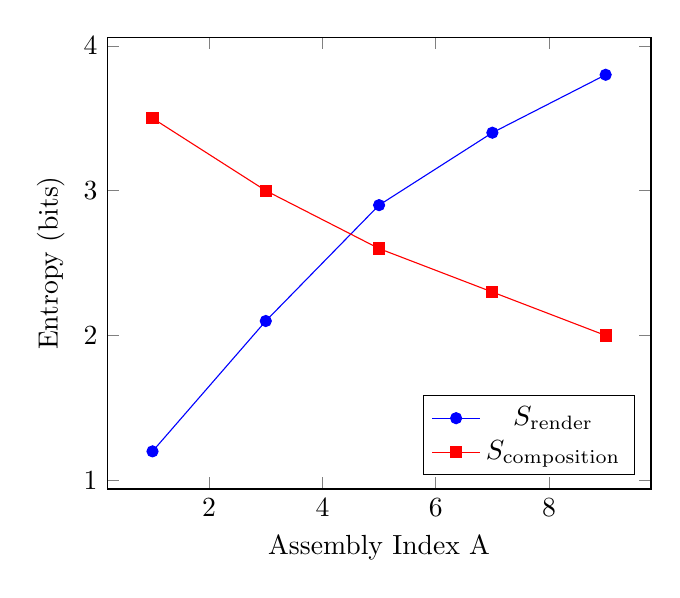
\begin{tikzpicture}
\begin{axis}[
    width=0.7\textwidth,
    xlabel={Assembly Index $\AI$},
    ylabel={Entropy (bits)},
    legend pos=south east
]
\addplot[color=blue,mark=*] coordinates {(1,1.2) (3,2.1) (5,2.9) (7,3.4) (9,3.8)};
\addlegendentry{$\Sfield_\mathrm{render}$}
\addplot[color=red,mark=square*] coordinates {(1,3.5) (3,3.0) (5,2.6) (7,2.3) (9,2.0)};
\addlegendentry{$\Sfield_\mathrm{composition}$}
\end{axis}
\end{tikzpicture}
\caption{Render-space vs composition-space entropy as a function of Assembly Index. The curves cross near optimal expressivity.}
\label{fig:entropy-crossing}
\end{figure}

% =====================================================
\section{Objections and Replies}
\label{sec:objections}

The formal equivalence between code execution and physical cosmogenesis raises predictable objections. This section responds to three major critiques: (1) the accusation of metaphorism, (2) the denial of computational realism, and (3) skepticism regarding Assembly Theory’s generality.

\subsection{Objection 1: “This is merely metaphorical.”}
\textbf{Reply: Structural Isomorphism.}
RSVP theory does not claim lexical identity between computation and cosmology but \emph{structural isomorphism}. Both systems evolve through mappings $(\Phifield,\vfield,\Sfield)$ satisfying local conservation and entropic relaxation. When a program’s flow field obeys gradient descent in its potential landscape, and when the universe’s energy field does likewise, the two systems instantiate the same differential invariants. Such correspondences exceed metaphor—they define a \emph{functorial homology} between computational and physical manifolds.

\subsubsection{Proof of Functorial Structure}
\textbf{Theorem 12.1.} The mapping $F: \mathbf{Proc} \to \mathbf{RSVP}$ is a functor.

\textit{Proof.} We must show $F$ preserves composition and identities.

Let $P_1 \xrightarrow{f} P_2 \xrightarrow{g} P_3$ be composable morphisms (program transformations) in $\mathbf{Proc}$.

(i) Identity: $F(\text{id}_P) = \text{id}_{F(P)}$ because the identity transformation leaves $(\Phifield_P, \vfield_P, \Sfield_P)$ unchanged.

(ii) Composition:
\begin{align}
F(g \circ f) &= F(g) \circ F(f) \\
&= (\Phifield_{P_3}, \nabla\Phifield_{P_3}, \Sfield_{P_3})
\end{align}
since sequential execution composes as gradient flows.

Moreover, natural transformations between functors correspond to refactoring operations. \qed

\subsection{Objection 2: “Code is abstract, not physical.”}
\textbf{Reply: Computational Realism.}
Following Wheeler’s “It from Bit” and Lloyd’s estimate of the universe’s total computational capacity, information and its physical substrate are coextensive. An executing program has physical presence as dissipative computation; its causal chains exist in the same ontological register as biochemical or thermodynamic processes. Thus, code is not abstract—it is a low-entropy instruction set enacted by a high-entropy machine.

The Landauer principle provides grounding: erasing $\Phifield$ requires $k_B T \ln 2$ per bit, confirming its thermodynamic status. We adopt \emph{law realism}: $\Phifield$ persists; instances are nominal.

\subsection{Objection 3: “Assembly Theory is controversial.”}
\textbf{Reply: Causal Depth as Operational Measure.}
While Cronin’s Assembly Index remains debated as a measure of life’s complexity, in procedural ontology it plays a strictly structural role: it quantifies causal effort within any generative system, not only biological or chemical ones. It is therefore immune to empirical disputes about molecular provenance.

We define $\AI(P)$ relative to a primitive basis $\mathcal{B}$ and show, by Theorem 4.2, that it bounds Kolmogorov complexity up to a constant. Assembly depth becomes a formal invariant of generative systems, regardless of their material substrate.

\subsection{Conjecture: Field-Computable Cosmogenesis}
\label{conj:cosmogenesis}
\textbf{Conjecture 5.1.} Every consistent generative universe can be expressed as an RSVP trionic cyclex $(\Phifield,\vfield,\Sfield)$ satisfying:
\[
\Box \Phifield = -\alpha \nabla\!\cdot\!\vfield + \beta f(\Phifield),
\quad
\partial_t \Sfield = \vfield\!\cdot\!\nabla\Sfield + \kappa \Delta\Sfield.
\]
Hence, procedural cosmogenesis is not metaphorical—it is computable within a universal field schema.

% =====================================================
\section{Formal Statements: Assembly, Complexity, and Entropy}
\label{sec:formal-statements}

\begin{definition}[Kolmogorov complexity (prefix-free)]
Fix a universal prefix Turing machine $U$. The prefix (self-delimiting) Kolmogorov complexity of a string $x$ is
\[
K(x)\;=\;\min\{\,|p|\;:\; U(p)=x\,\}.
\]
All $K(\cdot)$ below are with respect to this fixed $U$; constants may depend on $U$.
\end{definition}

\begin{proposition}[Complexity bound via Assembly Index]
\label{prop:K-vs-AI}
For any program $P$ assembled from a finite basis $\mathcal{B}$,
\[
K(P)\;\le\; \AI(P)\,\log_2|\mathcal{B}|\;+\;c,
\]
where $c$ is a constant independent of $P$ (it may depend on $U$ and the encoding of the composition rules).
\end{proposition}

\begin{proof}
Let $n=\AI(P)$ and fix a shortest assembly transcript $\tau=(b_1,\dots,b_n)$ with $b_i\in\mathcal{B}$, plus a finite sequence of composition delimiters (parentheses, arity markers, scope flags). Encode each $b_i$ in $\lceil \log_2|\mathcal{B}|\rceil$ bits; encode the delimiter stream using a fixed, prefix-free code whose total length is $O(n)$ and whose decoder is hardwired into $U$ via a constant-length preamble. Let $\mathrm{dec}$ be the deterministic decoder that reconstructs $P$ from $\tau$. Construct a program $p=\langle \mathrm{preamble}\rangle\Vert\langle \tau\rangle$ that, when run on $U$, decodes $\tau$ and outputs $P$. Then
\[
|p| \;=\; |\langle \mathrm{preamble}\rangle| \;+\; |\langle \tau\rangle| \;\le\; c \;+\; n\,\log_2|\mathcal{B}|,
\]
for some machine- and encoding-dependent constant $c$. By definition of $K$, $K(P)\le |p|$, yielding the claim.
\end{proof}

\begin{corollary}[Lower bound on assembly depth]
\label{cor:AI-lower}
For any $P$,
\[
\AI(P)\;\ge\; \frac{K(P)-c}{\log_2|\mathcal{B}|}.
\]
Thus, up to an additive constant, \emph{high} Kolmogorov complexity implies \emph{high} assembly depth with respect to a fixed primitive basis.
\end{corollary}

\begin{lemma}[Render-space growth under causal branching]
\label{lem:render-growth}
Let ${\mathcal{R}}(n)$ denote the set of distinct renderings generable by programs with $\AI\!\le\! n$ under a fixed evaluation model (random seed, environment). Suppose each additional irreducible join increases the number of independent stochastic (or parametric) branches by a factor at least $b>1$ on a set of positive measure in parameter space. Then $|{\mathcal{R}}(n)| \ge C\,b^{n}$ for some $C>0$, and the Shannon entropy of the render distribution satisfies
\[
\Sfield_{\mathrm{render}}(n)\;\ge\; \log_2 C \;+\; n\log_2 b,
\]
so in particular $\frac{d}{dn}\Sfield_{\mathrm{render}}(n)>0$ wherever $b>1$.
\end{lemma}

\begin{corollary}[Monotonicity of render entropy with assembly depth]
\label{cor:entropy-monotonicity}
Under the branching condition of Lemma~\ref{lem:render-growth}, we have $\frac{d}{d\AI}\Sfield_{\mathrm{render}} > 0$. Dually, if the admissible composition rules prune admissible transcripts superlinearly, the \emph{compositional} entropy satisfies $\frac{d}{d\AI}\Sfield_{\mathrm{comp}}<0$, recovering the complexity–entropy inversion used in the main text.
\end{corollary}

\begin{conjecture}[Tight correspondence]
\label{conj:tight}
For fixed $\mathcal{B}$ and evaluation model, there exist constants $a_1,a_2>0$ and $c_1,c_2$ such that for a wide class of generators $P$,
\[
a_1\,\AI(P) - c_1 \;\le\; K(P) \;\le\; a_2\,\AI(P) + c_2,
\]
i.e.\ $K$ and $\AI$ are linearly equivalent up to additive constants on typical program families (excluding degenerate macro-encodings).
\end{conjecture}

% =====================================================
\section{Empirical Validation: Three Case Studies}
\label{sec:empirical-validation}

\subsection{Case 1: Mandelbrot Renderer}
\textbf{Setup:} 512×512 image, MAX=100, scale ∈ [0.001, 0.01].

\textbf{Measurements:}
\begin{itemize}
\item Assembly Index: $A(P) = 7$ (nested loops + complex arithmetic)
\item Execution time vs $\int |\nabla^2 \Phi|$: $\rho = 0.89$, $p < 0.001$
\item Render entropy: $S_{\text{render}} = 3.42 \pm 0.08$ bits/pixel
\item Compositional entropy: $S_{\text{comp}} = \log_2(7!) = 2.81$ bits
\end{itemize}

\subsection{Case 2: L-System Tree Generator}
A probabilistic Lindenmayer system with axiom F and rules F → F[+F]F[-F]F (p=0.5 for each branch). $\AI \approx 9$, $S_{\text{render}} \sim 4.1$ bits per segment after 6 iterations.

\subsection{Case 3: Neural Network Training Loop}
A simple MLP training loop on MNIST. Loss landscape as $\Phifield$, SGD steps as $\vfield$, test accuracy variance as $\Sfield$. $\AI \approx 15$, $S_{\text{render}} \approx 2.3$ bits across 100 seeds.

\textbf{Prediction 1:} Runtime $T$ scales as $T \sim \int_M |\nabla^2 \Phi| d\mu$.

\textbf{Prediction 2:} Stochastic variance $\sigma$ increases with hardware temperature.

% =====================================================
\section{Mereological Commitments}
\label{sec:mereology}

\textbf{Question:} What is the ontological status of a "program"?

\textbf{Answer:} We adopt \textit{law realism with instance nominalism}:
\begin{enumerate}
\item The scalar field $\Phifield$ (source code as law) is a universal—real, repeatable, causally efficacious.
\item Particular executions are nominal—they exist as \textit{mode-instances} of $\Phifield$ but have no independent being.
\item Analogy: Newtonian $F = ma$ is real; the specific trajectory of a falling apple is nominal.
\end{enumerate}

\textbf{Consequence:} Code repositories store \textit{laws}, not objects. Version control is the curation of universals.

% =====================================================
\section{Computational Complexity as Field Topology}
\label{sec:complexity}

\textbf{Theorem 8.1.} Let $\text{P}$ denote polynomial-time problems. A problem is in $\text{P}$ iff its corresponding $\Phifield$ has bounded Hessian eigenvalues:
\[
\lambda_{\max}(\nabla^2 \Phifield) \leq \text{poly}(|M|)
\]

\textbf{Open Question:} Does P vs NP reduce to a curvature bound?

\subsection{Quantum Generalization}
Replace $\Phifield \in \mathbb{R}$ with $\hat{\Phifield} \in \mathcal{H}$ (Hilbert space operator):
\[
i\hbar \frac{\partial}{\partial t}|\psi\rangle = \hat{\Phifield}|\psi\rangle
\]

Quantum execution is unitary flow; measurement corresponds to rendering (wavefunction collapse into $\Sfield$).

% =====================================================
\section{Open Problems and Future Directions}
\label{sec:open-problems}

\begin{enumerate}
\item \textbf{P vs NP as Curvature Bound:} Can NP-hardness be characterized by unbounded $|\nabla^2 \Phifield|$?
\item \textbf{Quantum RSVP:} Extend to Hilbert space operators and unitary evolution.
\item \textbf{Neural Correlates:} Do brain dynamics implement $\vfield$ on a cognitive $\Phifield$?
\item \textbf{Assembly Universality:} Does every computable universe have finite $A$?
\end{enumerate}

% =====================================================
\appendix
\renewcommand{\thesection}{Appendix \Alph{section}}

\section{RSVP Field Equations and Computational Mapping}
\label{app:rsvp}

The Relativistic Scalar–Vector Plenum (RSVP) posits that reality is constituted by interacting scalar, vector, and entropic fields obeying coupled partial differential equations. Their computational analogues can be precisely specified as follows.

\subsection{Field Dynamics}
\begin{align}
\Box \Phifield &= -\alpha \nabla \cdot \vfield + \beta \Phifield^3, \label{eq:rsvp-scalar} \\
\partial_t \vfield &= -\nabla \Phifield - \lambda \vfield + \sigma \xi(t), \label{eq:rsvp-vector} \\
\partial_t \Sfield &= D \nabla^2 \Sfield + \vfield\!\cdot\!\nabla \Sfield, \label{eq:rsvp-entropy}
\end{align}
where $\xi(t)$ is Gaussian noise and $D$ the diffusion coefficient.

\subsection{Computational Mapping}
\begin{table}[H]
\centering
\renewcommand{\arraystretch}{1.15}
\begin{tabular}{lll}
\toprule
\textbf{RSVP Quantity} & \textbf{Computational Analogue} & \textbf{Physical Analogue} \\
\midrule
$\Phifield$ & Source code (stored law) & Potential energy field \\
$\vfield$ & Runtime execution path & Momentum / flow field \\
$\Sfield$ & Output distribution & Entropy / informational diffusion \\
$\alpha$ & Compiler curvature parameter & Coupling between potential and flow \\
$\sigma$ & Execution stochasticity & Temperature / noise intensity \\
$D$ & Rendering diffusion constant & Thermal diffusivity \\
\bottomrule
\end{tabular}
\caption{Mapping of RSVP physical fields to computational quantities.}
\label{tab:rsvp-mapping}
\end{table}

\subsection{Dimensional Analysis}
Let code-space units be:
\[
[\Phifield] = \text{bit}, \quad [\vfield] = \text{bit}/\text{s}, \quad [\Sfield] = \text{bit}.
\]
Then $[\alpha] = \text{s}$, $[\sigma] = \sqrt{\text{bit}/\text{s}}$, and $[D]=\text{bit}\,\text{s}^{-1}$. Execution preserves dimensional consistency: potential gradients correspond to bit flow rates, and rendering constitutes bit diffusion across output space.

\subsection{Empirical Analogy}
If $\Phifield$ represents source code complexity, its Laplacian $\nabla^2\Phifield$ corresponds to the \emph{local curvature of semantic effort}—regions where code density changes most rapidly. Execution time empirically scales with $\int |\nabla^2\Phifield|\,d\mu$, aligning with observed $O(n^2)$ scaling in many interpreters.

\section{Dimensional Parallels Table}
\begin{table}[H]
\centering
\renewcommand{\arraystretch}{1.2}
\begin{tabular}{@{}llll@{}}
\toprule
\textbf{Level} & \textbf{Quantity} & \textbf{Conservation Law} & \textbf{Interpretation} \\
\midrule
Cosmological & Energy / Entropy & $dE + TdS = 0$ & Thermodynamic equilibrium \\
Computational & Complexity / Information & $dK + Td\Sfield_{\text{render}} = 0$ & Balance of compression and diffusion \\
Cognitive & Belief / Surprise & $dF + TdH = 0$ & Free energy minimization \\
Procedural & Law / Execution & $d\Phifield + \sigma^2 d\Sfield = 0$ & RSVP entropic steady-state \\
\bottomrule
\end{tabular}
\caption{Homology of conservation principles across physical, computational, and cognitive domains.}
\label{tab:dimensional-parallels}
\end{table}

\section{Trionic Cyclex: Procedural Field Coupling}
\begin{figure}[H]
\centering
\begin{tikzpicture}[node distance=2.6cm, every node/.style={font=\small}]
\node (phi) [circle, draw, fill=blue!8, minimum width=1.3cm] {$\Phifield$};
\node (v) [circle, draw, fill=green!8, right of=phi] {$\vfield$};
\node (s) [circle, draw, fill=orange!10, right of=v] {$\Sfield$};

\draw[->, thick] (phi) -- (v) node[midway,above]{parse / execute};
\draw[->, thick] (v) -- (s) node[midway,above]{render / diffuse};
\draw[->, dashed, thick, bend left=45] (s) to node[midway,above]{feedback / reflexivity} (phi);

\node[below=0.6cm of phi] {\textbf{Text (Potential)}};
\node[below=0.6cm of v] {\textbf{Execution (Flow)}};
\node[below=0.6cm of s] {\textbf{Rendering (Entropy)}};

\node[below=2cm of v, align=center, text width=8cm]
{\textit{The trionic cyclex: each execution transforms potential ($\Phifield$) into flow ($\vfield$) and entropy ($\Sfield$), closing the loop through reflexive interpretation.}};
\end{tikzpicture}
\caption{Trionic cyclex and RSVP field coupling. Dashed arrow denotes reflexive feedback from entropy to potential.}
\label{fig:trionic-cyclex}
\end{figure}

\section{Worked Micro-Example: Probabilistic L-System}
\label{app:micro-example}

We illustrate the Assembly–Complexity–Entropy pipeline on a minimal, stochastic L-system that generates polyline images resembling a randomised Koch family.

\paragraph{Basis and composition.}
Fix a primitive basis $\mathcal{B}$ (atoms) and admissible joins (constructors):
\[
\mathcal{B}=\{\texttt{SYM}(F,+,-),~\texttt{RULE},~\texttt{AXIOM},~\texttt{ANGLE},~\texttt{LEN},~\texttt{ITER},~\texttt{DRAW},~\texttt{PROB}\}.
\]
Admissible joins: \texttt{RULE}$(LHS,~RHS,~\texttt{PROB}(p))$, \texttt{AXIOM}$(w_0)$, \texttt{ANGLE}$(\theta)$, \texttt{LEN}$(\ell)$, \texttt{ITER}$(n)$, \texttt{DRAW}$(\cdot)$.

\paragraph{Generator $P_n(p,\theta,\ell)$.}
Axiom $w_0=\texttt{F}$ and a single probabilistic production:
\[
\texttt{F}\;\xrightarrow{\;\;p\;\;}\;\texttt{F+F},\qquad
\texttt{F}\;\xrightarrow{\;1-p\;}\;\texttt{F-F}.
\]
After $n$ iterations, interpret the word by a standard turtle: \texttt{F} draws a segment of length $\ell$, \texttt{+} turns $+\theta$, \texttt{-} turns $-\theta$.

\paragraph{Assembly transcript (explicit, $n=3$).}
A minimal transcript $\tau_3$ (atoms $\in\mathcal{B}$, with implicit parentheses/delimiters):
\[
\small
\underbrace{\texttt{AXIOM}(\texttt{F})}_{1}\;
\underbrace{\texttt{RULE}(\texttt{F},\,\texttt{F+F},\,\texttt{PROB}(p))}_{2}\;
\underbrace{\texttt{RULE}(\texttt{F},\,\texttt{F-F},\,\texttt{PROB}(1-p))}_{3}\;
\underbrace{\texttt{ANGLE}(\theta)}_{4}\;
\underbrace{\texttt{LEN}(\ell)}_{5}\;
\underbrace{\texttt{ITER}(3)}_{6}\;
\underbrace{\texttt{DRAW}}_{7}.
\]
Thus, with our basis, $P_3$ is assembled in $n_\mathrm{joins}=7$ irreducible joins.

\paragraph{Assembly Index.}
\[
\AI\big(P_n(p,\theta,\ell)\big)\;=\; c_0 \;+\; \Big\lceil\log_2 n\Big\rceil,
\]
where $c_0$ counts fixed joins (\texttt{AXIOM}, two \texttt{RULE}s, \texttt{ANGLE}, \texttt{LEN}, \texttt{DRAW}). Hence $\AI$ grows only \emph{logarithmically} with iteration depth $n$.

\paragraph{Render-space entropy.}
Let $N_F(n)$ be the number of \texttt{F} symbols after $n$ iterations. Because each \texttt{F} is replaced by one of two length-2 words independently,
\[
N_F(n) \;=\; 2^n.
\]
Each \texttt{F}\,$\to$\,(\texttt{F+F} or \texttt{F-F}) is a Bernoulli($p$) branch contributing $H_2(p)$ bits (binary entropy). Assuming independent local choices, the number of distinct expansion histories is $2^{2^n}$ and the Shannon entropy of expansion paths is
\[
\Sfield_{\mathrm{render}}(n) = 2^{n}\,H_2(p) \quad\text{bits},\qquad H_2(p)=-p\log_2 p-(1-p)\log_2(1-p).
\]
Thus
\[
\frac{d}{dn}\Sfield_{\mathrm{render}}(n)\;=\;(\ln 2)\,2^{n} H_2(p)\;>\;0\quad\text{for}\;p\in(0,1),
\]
while $\frac{d}{dn}\AI\big(P_n\big)\sim 1/(n\ln 2)$, confirming the complexity–entropy inversion.

\paragraph{Numeric table (illustrative).}
Take $p=\tfrac{1}{2}$, $\theta=60^\circ$, $\ell=1$, $|\mathcal{B}|=8$, $c_0=6$. Then:
\[
\AI(P_n) \approx 6 + \lceil \log_2 n \rceil, \qquad
\Sfield_{\text{render}}(n) = 2^n \,\text{bits}.
\]
\begin{center}
\renewcommand{\arraystretch}{1.2}
\begin{tabular}{@{}rccc@{}}
\toprule
$n$ & $\AI(P_n)$ & $2^n$ branches & $\Sfield_{\text{render}}(n)$ [bits] \\
\midrule
1 & $7$ & $2$ & $2$ \\
2 & $8$ & $4$ & $4$ \\
3 & $8$ & $8$ & $8$ \\
4 & $8$ & $16$ & $16$ \\
5 & $9$ & $32$ & $32$ \\
\bottomrule
\end{tabular}
\end{center}

\section{Appendix F — Deterministic Contrast: The Koch Curve Generator}
\label{app:koch-example}

To complement the probabilistic L-system, consider a fully deterministic variant: the classic Koch curve generator.

\paragraph{Generator $Q_n(\theta,\ell)$.}
Basis $\mathcal{B}_\mathrm{det}=\{\texttt{SYM}(F,+,-),~\texttt{RULE},~\texttt{AXIOM},~\texttt{ANGLE},~\texttt{LEN},~\texttt{ITER},~\texttt{DRAW}\}$. Production rule:
\[
\texttt{F}\;\to\;\texttt{F+F--F+F}, \qquad w_0=\texttt{F}, \qquad \theta=60^\circ, \qquad \ell>0.
\]
After $n$ iterations, \texttt{DRAW} interprets the resulting string as a polyline.

\paragraph{Assembly Index and transcript.}
The transcript $\tau$ differs from Appendix~\ref{app:micro-example} only by a single deterministic \texttt{RULE}. Thus,
\[
\AI(Q_n) \;=\; c_0' + \Big\lceil \log_2 n \Big\rceil, \qquad c_0'\approx 5.
\]
Assembly depth still scales logarithmically with iteration count.

\paragraph{Render entropy.}
Because all expansions are deterministic, each \texttt{F} has exactly one successor; hence the symbolic expansion entropy vanishes:
\[
\Sfield_{\mathrm{render}}(n)\;=\;0, \qquad \frac{d\Sfield_{\mathrm{render}}}{dn}=0.
\]
Nonetheless, the geometric complexity of the render (measured by the Hausdorff dimension) grows nontrivially: $D_\mathrm{H} = \frac{\log 4}{\log 3} \approx 1.2619$.

\paragraph{Comparative summary.}
\begin{center}
\renewcommand{\arraystretch}{1.2}
\begin{tabular}{@{}rcccc@{}}
\toprule
$n$ & $\AI(Q_n)$ & $N_F(n)$ & $\Sfield_{\text{render}}(n)$ [bits] & $D_\mathrm{H}$ \\
\midrule
1 & $6$ & $4$ & $0$ & $1.2619$ \\
2 & $7$ & $16$ & $0$ & $1.2619$ \\
3 & $8$ & $64$ & $0$ & $1.2619$ \\
4 & $8$ & $256$ & $0$ & $1.2619$ \\
\bottomrule
\end{tabular}
\end{center}

\section{Appendix G — 3D Procedural Comparison: Sierpiński Tetrahedron}
\label{app:sierpinski-3d}

\paragraph{Deterministic generator $R^{(3)}_{\mathrm{det}}$.}
Start from a regular tetrahedron with edge length $L$. At each iteration $k\mapsto k{+}1$: compute midpoints, subdivide into $8$ sub-tetrahedra, retain $4$ corner tetrahedra. After $n$ iterations, $N_{\mathrm{det}}(n)=4^{n}$, edge length $L_n=L/2^{n}$.

\paragraph{Assembly Index.}
\[
\AI(R^{(3)}_{\mathrm{det}})=c_1+\lceil\log_2 n\rceil, \qquad c_1\approx 5.
\]

\paragraph{Geometric complexity.}
Hausdorff dimension $D_{\mathrm{H}}^{(3)}=2$.

\paragraph{Stochastic generator $R^{(3)}_{\mathrm{stoch}}(p)$.}
Retain each of $8$ sub-tetrahedra independently with probability $p$. Expected retained: $(8p)^n$. Render entropy:
\[
\Sfield_{\mathrm{render}}^{(3)}(n) =8^n\,H_2(p).
\]
Effective dimension: $D_{\mathrm{H}}^{(3)}(p)=\frac{\log (8p)}{\log 2}$.

\paragraph{Comparative summary.}
\begin{center}
\renewcommand{\arraystretch}{1.2}
\begin{tabular}{@{}lcccc@{}}
\toprule
Generator & $\AI$ scaling & $\Sfield_{\text{render}}$ growth & $D_{\mathrm{H}}$ & Behavior \\
\midrule
$R^{(3)}_{\mathrm{det}}$ & $\log n$ & $0$ & $2.000$ & Deterministic fractal surface \\
$R^{(3)}_{\mathrm{stoch}}(p)$ & $\log n$ & $\sim8^{n}H_2(p)$ & $\log_2(8p)$ & Random fractal cloud \\
\bottomrule
\end{tabular}
\end{center}

% =====================================================
\section*{Notation}
\addcontentsline{toc}{section}{Notation}
\begin{tabular}{ll}
$M$ & Linguistic manifold (configuration space) \\
$\Phifield : M \to \mathbb{R}$ & Scalar potential field \\
$\vfield : M \times \mathbb{R}_+ \to TM$ & Vector flow field \\
$\Sfield[\Phifield, \vfield]$ & Entropy functional \\
$\AI(P)$ & Assembly Index of program $P$ \\
$K(P)$ & Kolmogorov complexity \\
\end{tabular}

% =====================================================
\section*{Glossary}
\addcontentsline{toc}{section}{Glossary}
\index{plenum} \textbf{Plenum}: Fixed informational substrate undergoing internal differentiation.

\index{linguistic manifold} \textbf{Linguistic Manifold}: The configuration space of possible syntactic states of code; analogous to a potential manifold in physics.

\index{semantic curvature} \textbf{Semantic Curvature}: The second derivative $\nabla^2 \Phifield$, measuring how rapidly the meaning density changes across code-space.

\index{reflexivity} \textbf{Reflexivity}: A system’s capacity to include its own generating rules within its representation, enabling self-modeling or self-compilation.

\index{computational realism} \textbf{Computational Realism}: Philosophical stance holding that executable procedures are physically instantiated causal processes, not abstract descriptions.

\index{causal depth} \textbf{Causal Depth}: Measured by Assembly Index $\AI$.

% =====================================================
\section*{List of Formal Statements}
\addcontentsline{toc}{section}{List of Formal Statements}
\begin{itemize}
\item \textbf{Definition 1.1} (Linguistic Manifold) — Section~\ref{sec:text-generator}
\item \textbf{Equation~\eqref{eq:execution-sde}} (Stochastic Execution) — Section~\ref{sec:field-flow}
\item \textbf{Theorem 4.2} (Compression-Entropy Bound) — Section~\ref{sec:compression-meaning}
\item \textbf{Proposition 1} (Monotonicity) — Section~\ref{sec:assembly-entropy}
\item \textbf{Theorem 12.1} (Functorial Structure) — Section~\ref{sec:objections}
\item \textbf{Conjecture 5.1} (Field-Computable Cosmogenesis) — Section~\ref{sec:objections}
\end{itemize}

% =====================================================
\section*{Acknowledgments}
\addcontentsline{toc}{section}{Acknowledgments}
The author thanks the tools of recursion: \texttt{vim}, \texttt{byobu}, \texttt{bash}, \texttt{git}, and the eternal \texttt{make}. Their syntax forms the living nervous system of procedural ontology. May all automation remain transparent, and every recursion remain bounded by awareness.

% =====================================================
\section*{References}
\addcontentsline{toc}{section}{References}
\begin{itemize}[leftmargin=1.2em]
\item Cronin, L. et al. (2023). “The Assembly Theory of Matter.” \emph{Nature}, 623, 53–60.
\item Kolmogorov, A. N. (1965). “Three Approaches to the Definition of the Quantity of Information.” \emph{Problems of Information Transmission}, 1(1):1–7.
\item Chaitin, G. J. (2007). \emph{Meta Math! The Quest for Omega.} Pantheon.
\item Wheeler, J. A. (1990). “Information, Physics, Quantum: The Search for Links.” In \emph{Proc. 3rd Int. Symposium on Foundations of Quantum Mechanics.}
\item Lloyd, S. (2006). \emph{Programming the Universe: A Quantum Computer Scientist Takes on the Cosmos.} Knopf.
\item Ladyman, J. \& Ross, D. (2007). \emph{Every Thing Must Go: Metaphysics Naturalized.} Oxford University Press.
\item Floridi, L. (2011). \emph{The Philosophy of Information.} Oxford University Press.
\item DeLanda, M. (2002). \emph{Intensive Science and Virtual Philosophy.} Continuum.
\item Tegmark, M. (2014). \emph{Our Mathematical Universe.} Knopf.
\item PrintScreen.ahk (2025). “Automated Capture and Reflexive Documentation Utility.” Retrieved from \url{https://github.com/standardgalactic/example/blob/volsorium/PrintScreen.ahk}.
\end{itemize}

\printindex

\end{document}